\documentclass[12pt]{article}
\usepackage[none]{hyphenat}
\usepackage{amsmath}
\usepackage{float}
\usepackage{graphicx}
\usepackage{atbegshi}
\AtBeginDocument{\AtBeginShipoutNext{\AtBeginShipoutDiscard}}
\newcommand{\solution}{\noindent \textbf{Solution: }}
\providecommand{\brak}[1]{\ensuremath{\left(#1\right)}}
\newcommand{\myvec}[1]{\ensuremath{\begin{pmatrix}#1\end{pmatrix}}}
\let\vec\mathbf
\begin{document}
\graphicspath{{./Documents}{./figs}}
\begin{center}
	\title{\textbf{Straight Lines}}
	\date{\vspace{-5ex}}
	\maketitle
\end{center}
\setcounter{page}{1}
\section*{11$ ^{th} $ Maths - Chapter 10}
The following problem is question 13 from exercise 10.3:
\begin{enumerate}
	\item Find the equation of the right bisector of the
 line segment joining the points (3, 4) and (–1, 2).
\end{enumerate}
\solution \\
Given that
\begin{align}
   \vec{A} &= \myvec{3\\\\4}\\
   \vec{B} &= \myvec{-1\\\\2}\\
\end{align}
The midpoint is given by
\begin{align}
     \vec{M} &= \frac{1}{2}(\vec{OA} + \vec{OB})\\
   & = \frac{1}{2}\myvec{3 - 1\\\\4 + 2}\\
   & = \myvec{1\\\\3}
\end{align}
The direction vector is given by
\begin{align}
    \vec{d} &= (\vec{B} - \vec{A})\\
    & = \myvec{ 2 -4 \\\\\ -1 -3 }\\
    & = \myvec{-2 \\\\ -4}
\end{align}
The slope of the perpendicular bisector is the negative reciprocal of the slope of line segment
\begin{align}
    & = \frac{-2}{-4}\\
    & = \frac{1}{2}
\end{align}
So, The slope of the perpendicular bisector is -2\\
Equation of line
\begin{align}
    ( y - y_1 ) &= m ( x - x_1)\\
    ( y - 3 ) &= -2 ( x - 1 )\\
    y &= - 2x + 5\\
    2x + y &= 5
\end{align}
\begin{figure}[H]
  \centering
  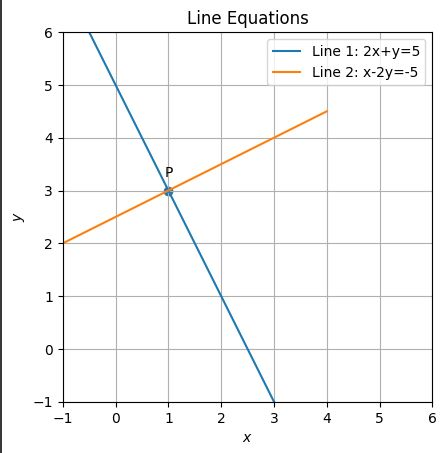
\includegraphics[width=\columnwidth]{figs/graph.jpg}
  \caption{Graph}
  \label{fig:pic}
\end{figure}
\end{document}
